% TU Delft beamer template
% Author: Erwin Walraven (initial version was created by Maarten Abbink)
% Delft Universiy of Technology

\documentclass{beamer}
\usepackage{amsmath}
\usepackage{amsfonts}
\usepackage{amsthm}
\usepackage{mathtools}
\usepackage[english]{babel}
\usepackage{calc}
\usepackage[absolute,overlay]{textpos}
\usepackage{graphicx}
\usepackage{subfig}
\usepackage{comment}
%\usepackage{tikz}
\usepackage{wasysym}
\usepackage{gensymb}
\usepackage{amssymb}
\usepackage{nccmath}
\usepackage{empheq}
\usepackage{xcolor}
\usepackage{relsize}
%\usepackage{apalike}
\usepackage[utf8]{inputenc}
\usepackage{multimedia}
\usepackage{media9}
%\usepackage{hyperref}.
\usepackage[table]{colortbl}


\usepackage{arydshln}


\makeatletter
\renewcommand*\env@matrix[1][*\c@MaxMatrixCols c]{%
	\hskip -\arraycolsep
	\let\@ifnextchar\new@ifnextchar
	\array{#1}}
\makeatother


\newcommand*\widefbox[1]{\fbox{\hspace{1em}#1\hspace{1em}}}
%\useoutertheme{miniframes}

%\usefonttheme[onlymath]{serif}



\setbeamertemplate{navigation symbols}{} % remove navigation symbols
\mode<presentation>{\usetheme{tud}}


%\ExecuteBibliographyOptions{parentracker=false}



% BIB SETTINGS
%\usepackage[backend=bibtex,firstinits=true,maxnames=30,maxcitenames=20,url=false,style=authoryear]{biblatex}
%\bibliography{MyBib}
%\addbibresource{MyBib.bib}
%\setlength\bibitemsep{0.3cm} % space between entries in the reference list
%\renewcommand{\bibfont}{\normalfont\scriptsize}
%\setbeamerfont{footnote}{size=\tiny}
%\makeatletter
%\renewcommand{\cite}[1]{\footnote<.->[frame][{\fullcite{#1}}]}
%\renewcommand{\cite}[1]{$[$\cite{#1}$]$}


% Insert frame before each subsection (requires 2 latex runs)
\AtBeginSection {
	\begin{frame}<beamer>[noframenumbering] \frametitle{\titleSubsec}
		\tableofcontents[currentsection,currentsubsection]  % Generation of the Table of Contents
	\end{frame}
}

% Define the title of each inserted pre-subsection frame
\newcommand*\titleSubsec{Outline}
% Define the title of the "Table of Contents" frame
\newcommand*\titleTOC{Outline}

\graphicspath{ {./images/} } 

\title[PhD meeting: Planning and Control]{PhD meeting \vspace{15pt}}
\institute[]{Istituto Italiano di Tecnologia, Genova, Italy \vspace{20pt}}
\author{Octavio A. Villarreal Maga\~na \vspace{20pt}} %\scriptsize Committee:  \\ Prof.Dr.Ir. Nathan van de Wouw (TUDelft, supervisor) \\ \vspace{1.5pt} \hspace{-11pt}Prof.Dr.Ir. Emmanuel Detournay (UMN, supervisor) \\ \vspace{-2.5pt} \hspace{-74pt}Dr.Ir. Manuel Mazo Jr. (TUDelft)}
\date{March 28th, 2017}

\begin{document}
{
\setbeamertemplate{footline}{\usebeamertemplate*{minimal footline}}
\frame{\titlepage}
\begin{frame}\frametitle{\titleTOC}
	\tableofcontents
\end{frame}
}

{\setbeamertemplate{footline}{\usebeamertemplate*{minimal footline}}
}

\section{Summary of work done}

\begin{frame}{Anticipation of an event}
	\begin{itemize}\setlength\itemsep{3em}
		\item Solved the problem of an anticipated event (90 \%)
		\item Worked on Introduction to Convex Optimization exam
		\item Studied Roy's course to give the exam this week
	\end{itemize}
\end{frame}

\section{Solution of anticipated event and approach to delayed event}

\begin{frame}{Method to solve anticipated event}
\begin{itemize}
\item Detect when a touchdown or lift-off occurs (just related to reference for now)
\item Update list of current events [Shahbazi 2015]
\item Compute next list events according to new state of current events
\end{itemize}
\begin{table}[]
\centering
\label{my-label}
\resizebox{\textwidth}{!}{\begin{tabular}{|l|l|l|l|l|l|l|l|l|}
\hline
$k$ & $g_1(k)$ & $g_2(k)$ & $g_3(k)$ & $g_4(k)$ & $l_1(k)$ & $l_2(k)$ & $l_3(k)$ & $l_4(k)$ \\ \hline
0   & 0        & 0        & 0        & 0        & 0        & 0        & 0        & 0        \\ \hline
1   & \cellcolor{red!25}2.4 (2.3)      & 3.6      & 3.6      & 2.4,     & 1.4      & 2.6      & 2.6      & 1.4      \\ \hline
\rowcolor{red!25}2   & 4.8      & 6        & 6        & 4.8      & 3.8      & 5        & 5        & 3.8      \\ \hline
3   & 7.2      & 8.4      & 8.4      & 7.2      & 6.2      & 7.4      & 7.4      & 6.2      \\ \hline
4   & 9.6      & 10.8     & 10.8     & 9.6      & 8.6      & 9.8      & 9.8      & 8.6      \\ \hline
5   & 12       & 13.2     & 13.2     & 12       & 11       & 12.2     & 12.2     & 11       \\ \hline
\end{tabular}}
\end{table}

\end{frame}
\begin{frame}{Simulation parameters}
\begin{itemize}\setlength\itemsep{3em}
\item Simulated a slower convergence in the oscillator equations (i.e., lowered the gains $\alpha = 0.05$ and $\beta = 0.05$)
\item Gait parameters:
\begin{itemize}
\item $G={1}\prec {2} \prec {3} \prec {4}$
\item $D_f = 0.8$
\item $S_f = 1/3 \frac{1}{s}$
\item $\Delta = [0.15,0.15,0.15,0.15]$
\end{itemize}
\end{itemize}

\end{frame}

\begin{frame}{Duty factor without feedback}
\vspace{-1cm}
	\begin{figure}[ht]\centering
		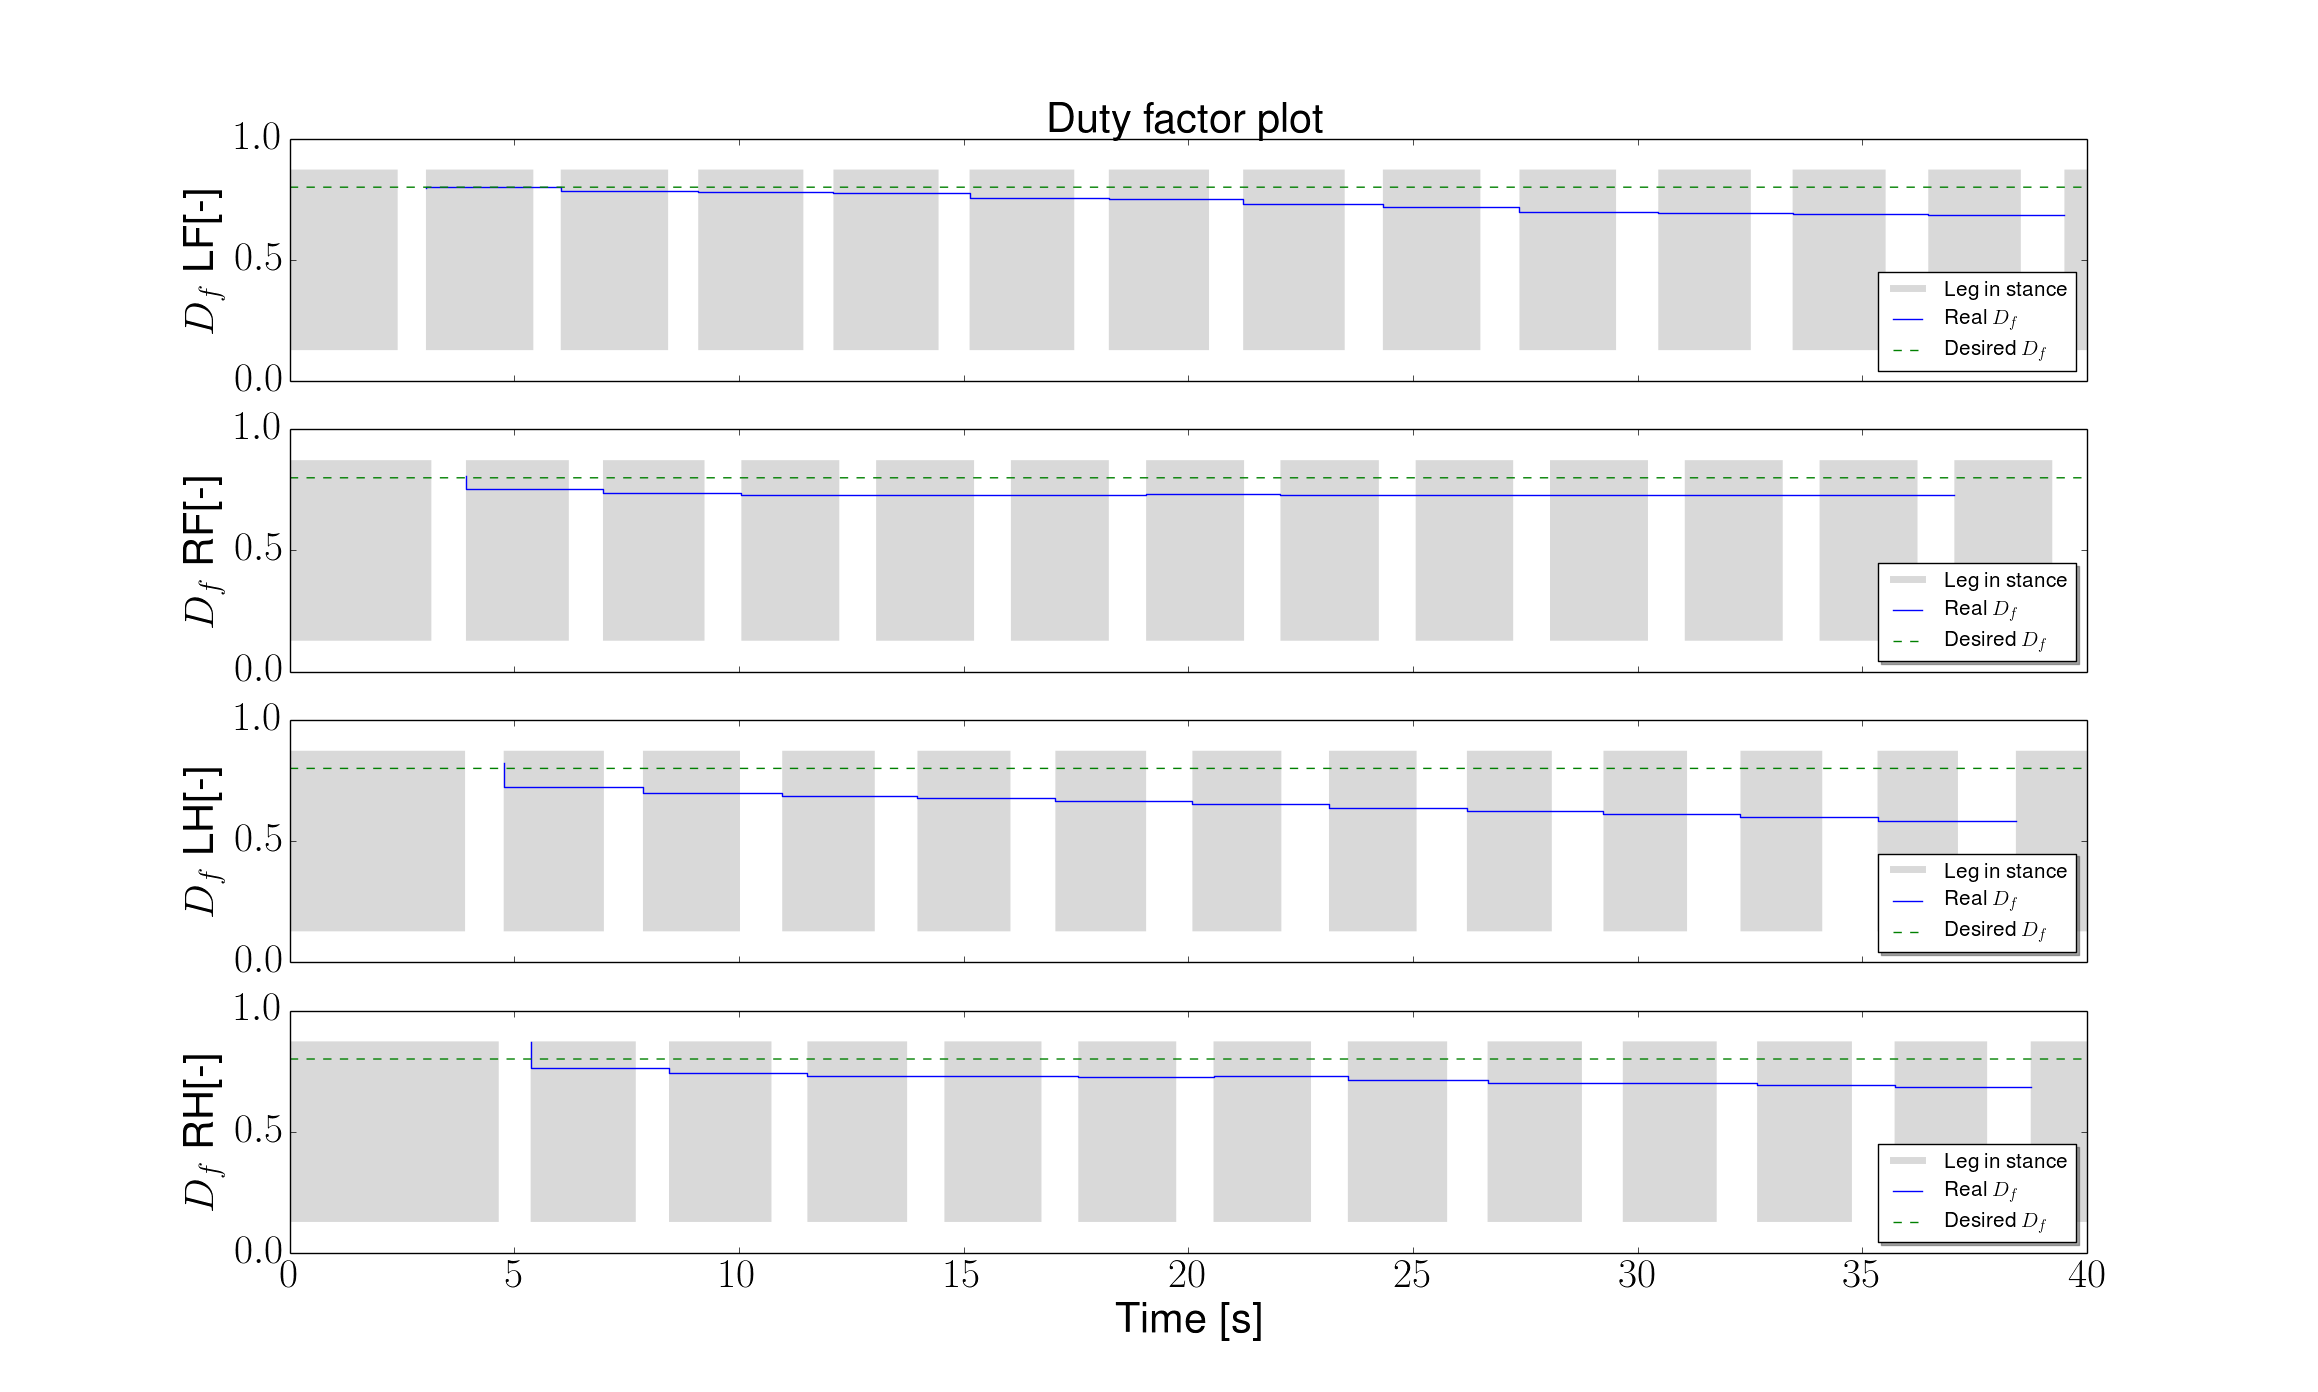
\includegraphics[width=1.1\textwidth]{images/DutyFactorFF.png}
	\end{figure}\vspace{-20pt}
\end{frame}

\begin{frame}{Duty factor with feedback}
\vspace{-1cm}
	\begin{figure}[ht]\centering
		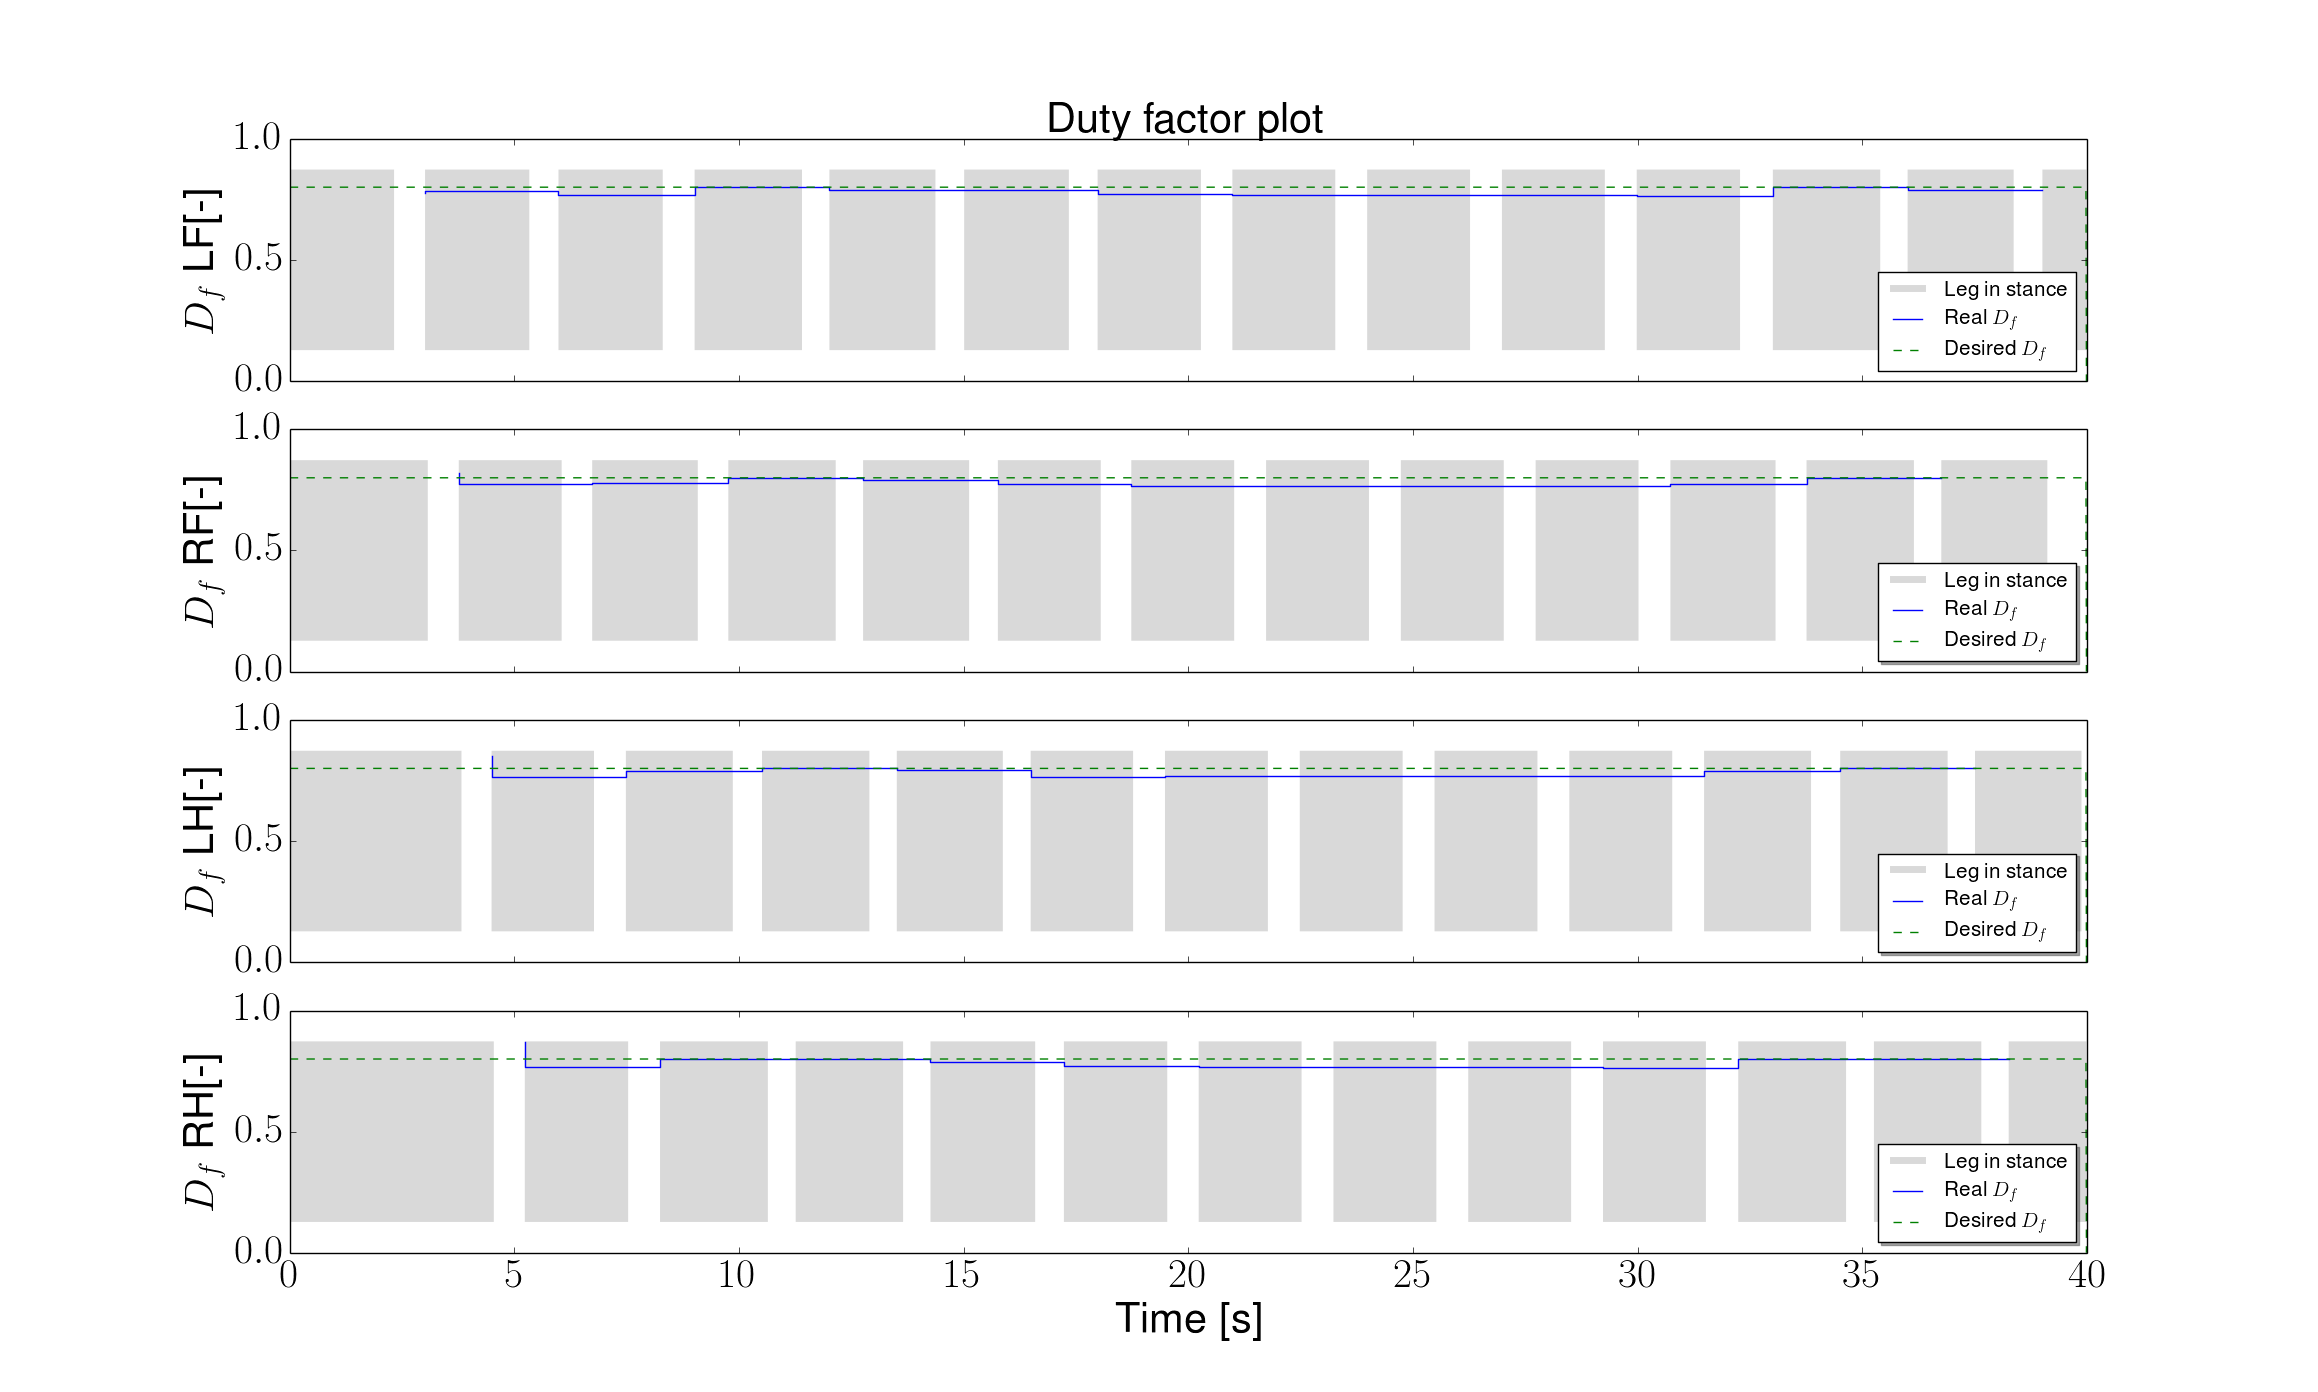
\includegraphics[width=1.1\textwidth]{images/DutyFactor.png}
	\end{figure}\vspace{-20pt}
\end{frame}

\begin{frame}{Position and angular frequency of the legs without feedback}
\begin{center}
	\begin{figure}[ht]\centering
		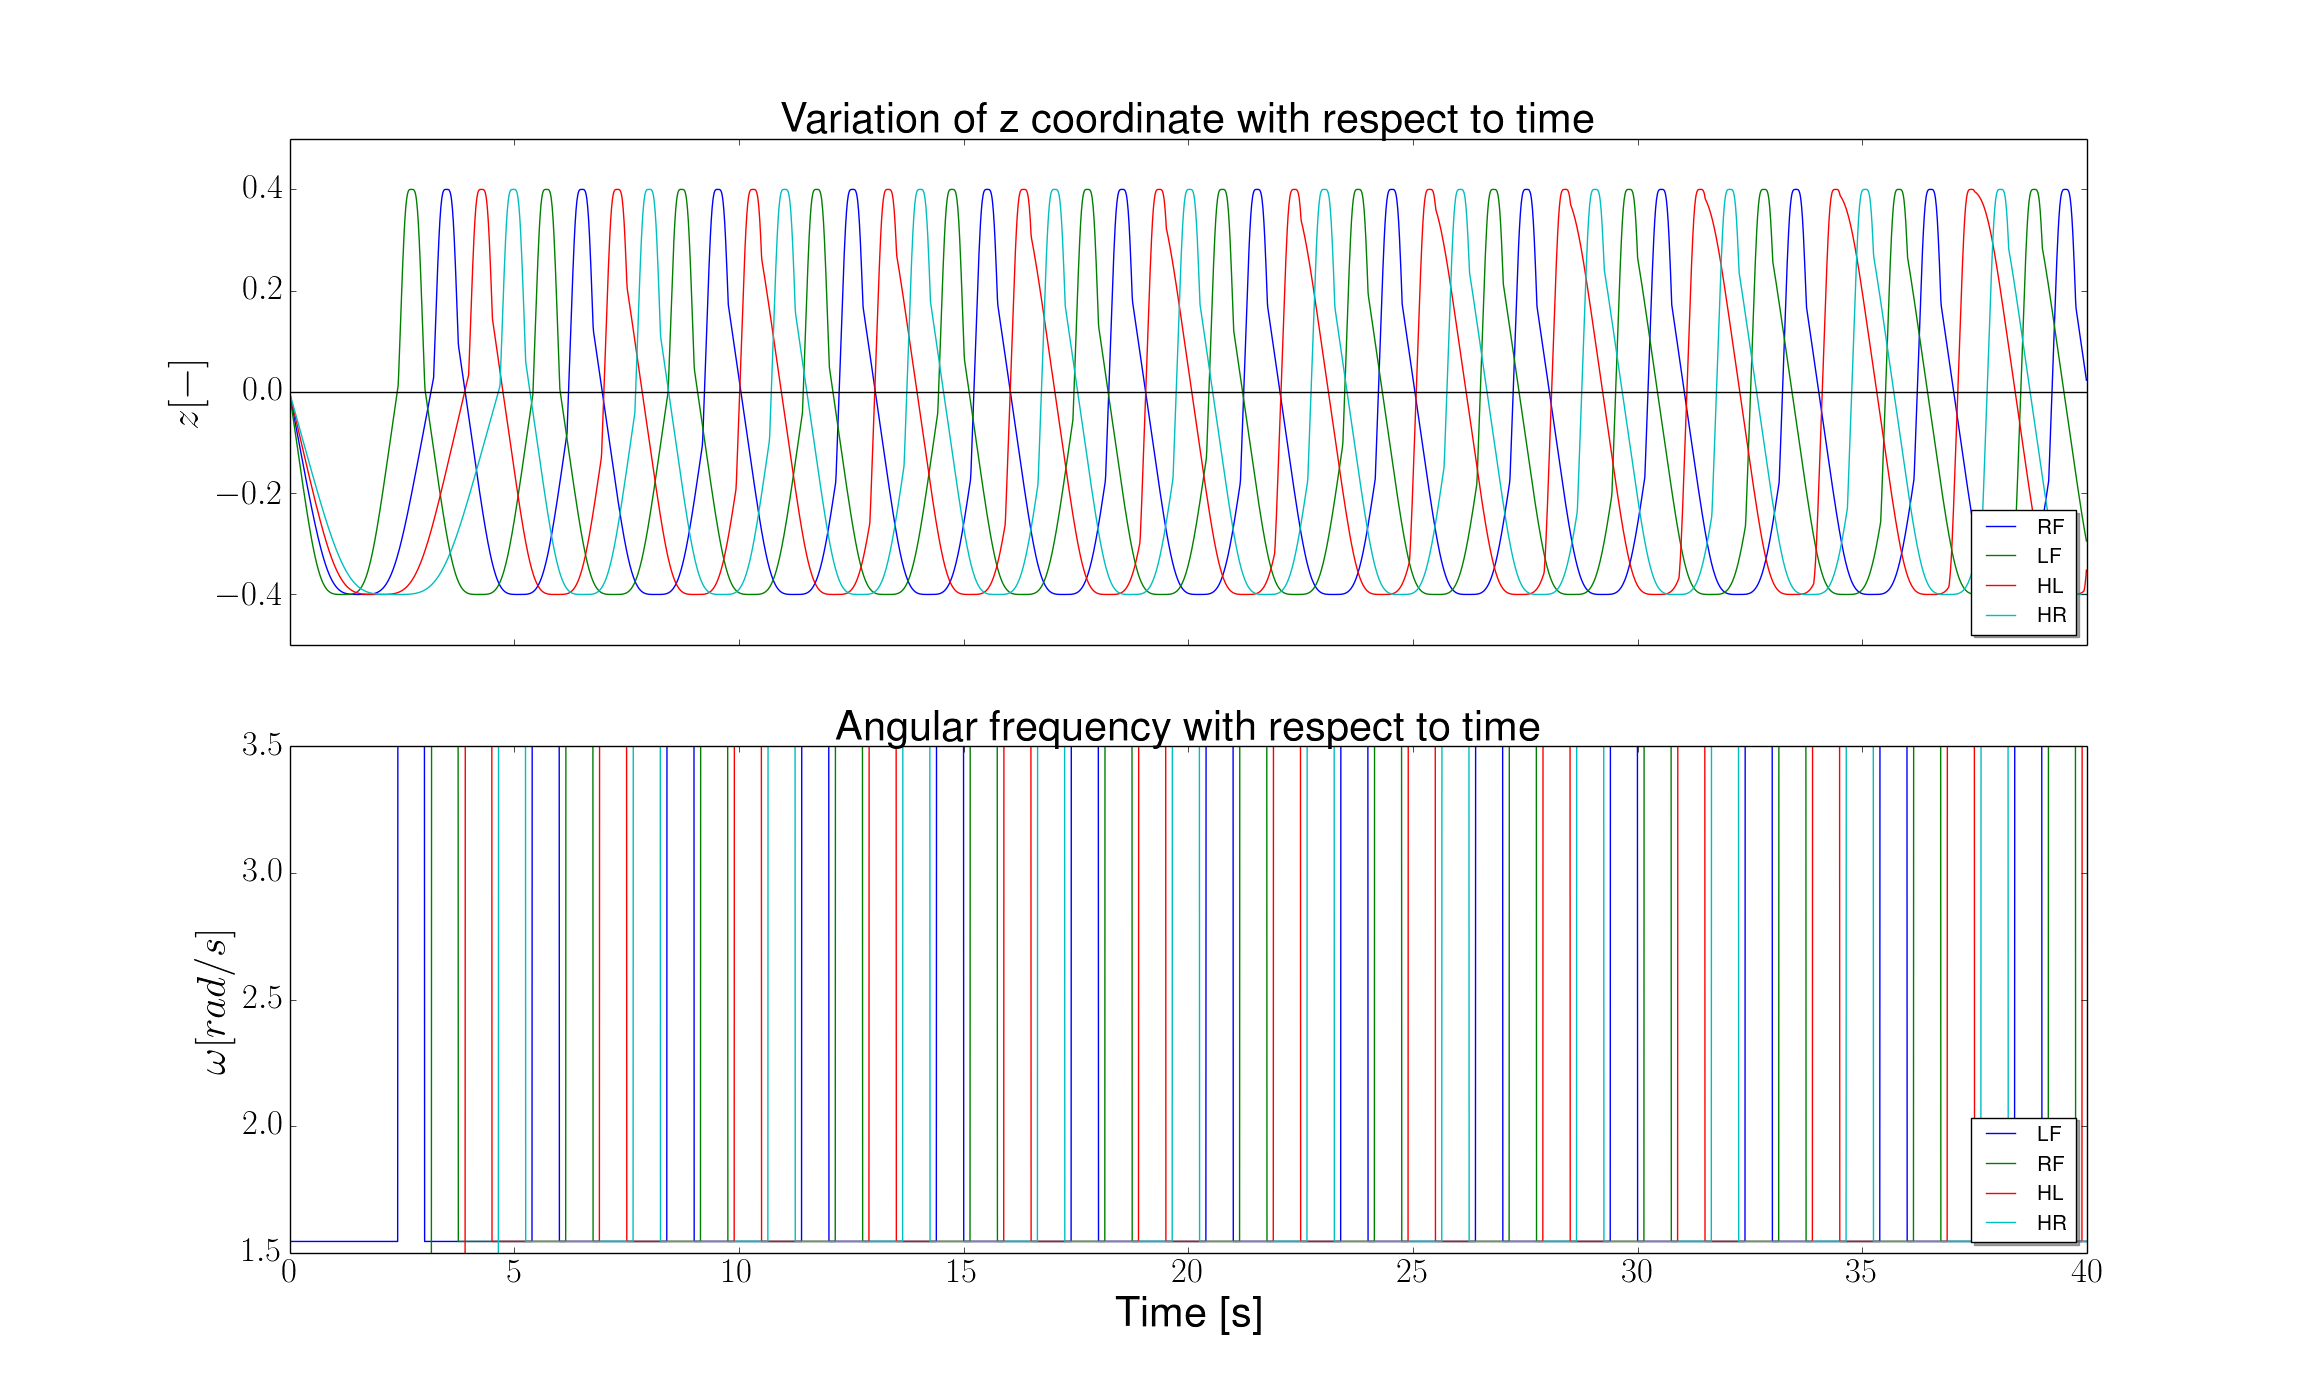
\includegraphics[width=1.1\textwidth]{images/HeightTimeFF.png}
	\end{figure}\vspace{-20pt}
\end{center}
\end{frame}

\begin{frame}{Position and angular frequency of the legs with feedback}
\begin{center}
	\begin{figure}[ht]\centering
		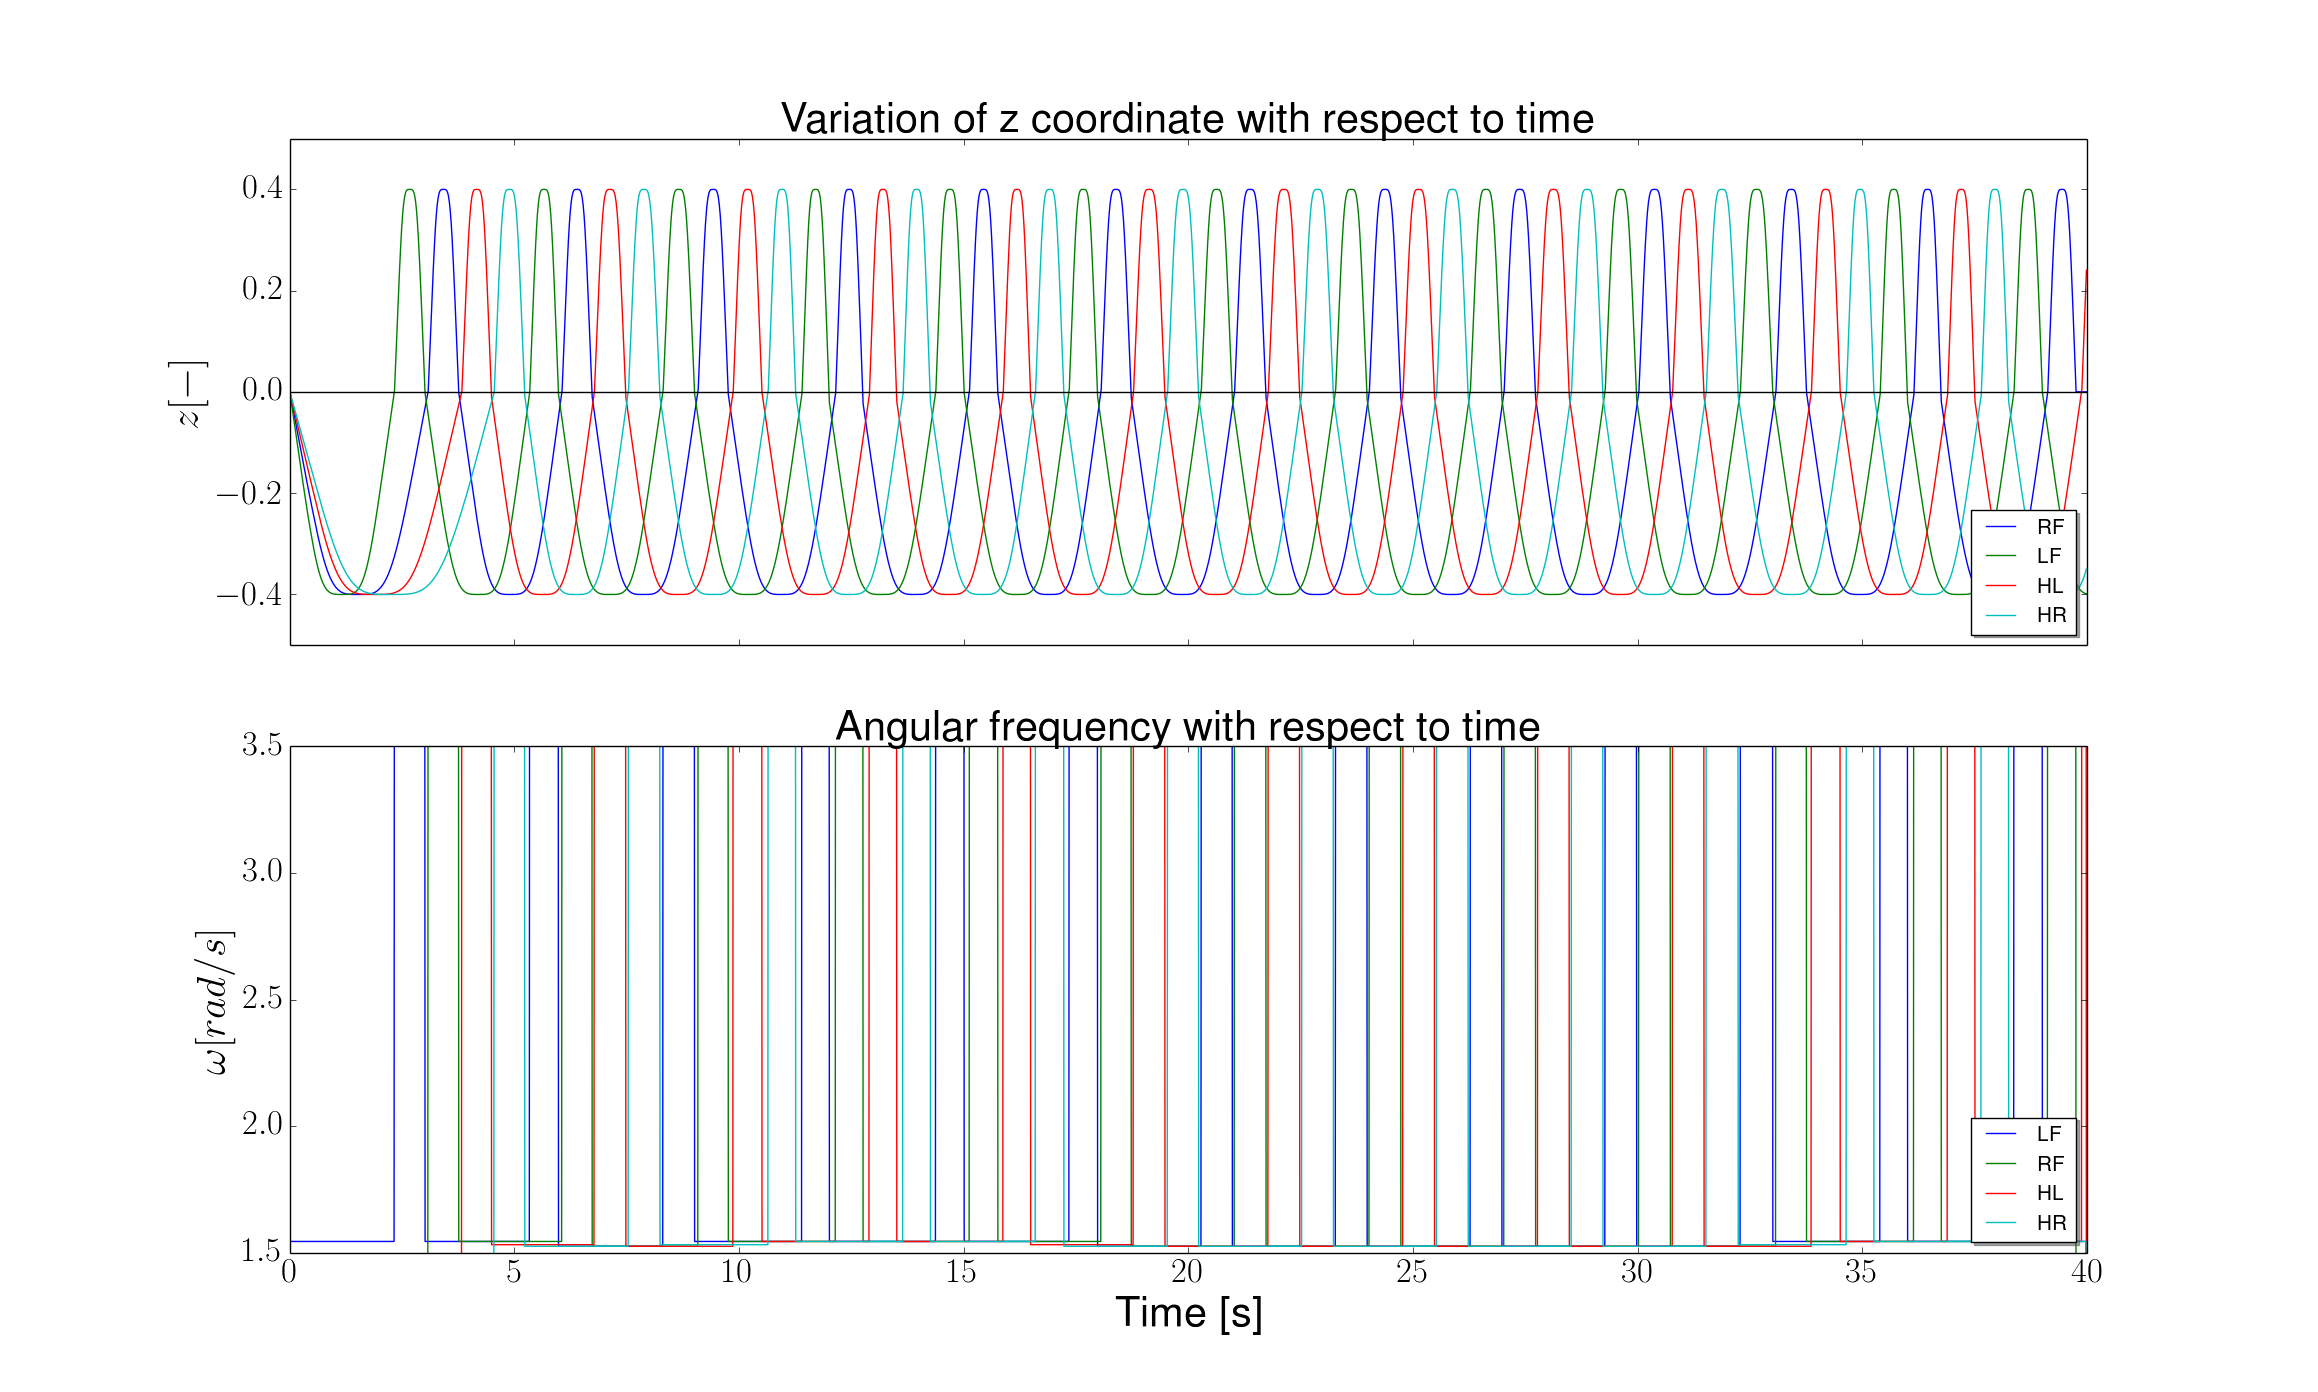
\includegraphics[width=1.1\textwidth]{images/HeightTime.png}
	\end{figure}\vspace{-20pt}
\end{center}
\end{frame}
\section{Summer schools and workshops}
\begin{frame}
	\begin{itemize}\setlength\itemsep{3em}
		\item Numerical methods for optimal control problems (NUMOC) (Rome, Italy, June 19th-23rd)
		\item Machine Learning Crash Course (Genova, Italy, June 26th-30th)
		\item BMVA Computer Vision Summer School (Lincoln, UK, July 3rd-7th)
	\end{itemize}
\end{frame}

\begin{frame}{Approach delayed event}
\begin{itemize}\setlength\itemsep{3em}
	\item Predict the new time of the delayed event based on sensor information and model [Shahbazi 2016]
	\item Use Model Predictive Control approach to ensure that the legs fulfill an specified schedule (not sure if this is the right way, main problem: disturbance model) [De Schutter 2001]
	\item On-off approach: wait until the leg reaches an event and update list of events 
\end{itemize}
\end{frame}


\section{Further work}


\begin{frame}{Further work}
	\begin{itemize}\setlength\itemsep{3em}
		\item Use the proposed strategy in the current framework
		\item Consider a delay in the occurrence of an event (prediction)
		\item Give Roy's exam (this week)
	\end{itemize}
\end{frame}

\begin{frame}
 \hspace{2cm} Thank you. Questions or comments?
\end{frame}





\end{document}
